% !TEX root = Thesis.tex

\section{Case Studies}

Text text text

\subsection{Interview Technique}
%TODO evtl kürzer fassen
In order to complement theoretical findings from literature research, expert interviews have been conducted. A structure for the interviews has been defined (see appendix). In this way, statements from different experts can be compared and evaluated, which allows for a comprehensive review. Even though interviewees may share their native language (German) with the interviewer, interviews have always been conducted in English. Thus, any inaccuracies that may occur during translating the statements were prevented and comparability of interviews has been improved.

The interviews were held remotely, either via an Internet VoIP-Service such as Skype, or via using WebEx, the standard communication platform used at T-Systems when interviewing employees of this company. Considering the often tight schedules of experts in their fields, the duration of interviews was planned to be 45 minutes.

To further document the interviews and the steps leading up to them as well as the steps of refinement that follow, a process (see figure \ref{fig:Intprocess}) has been defined and adhered to. 

\vspace{3mm}
\begin{figure}[htb]
	\centering
	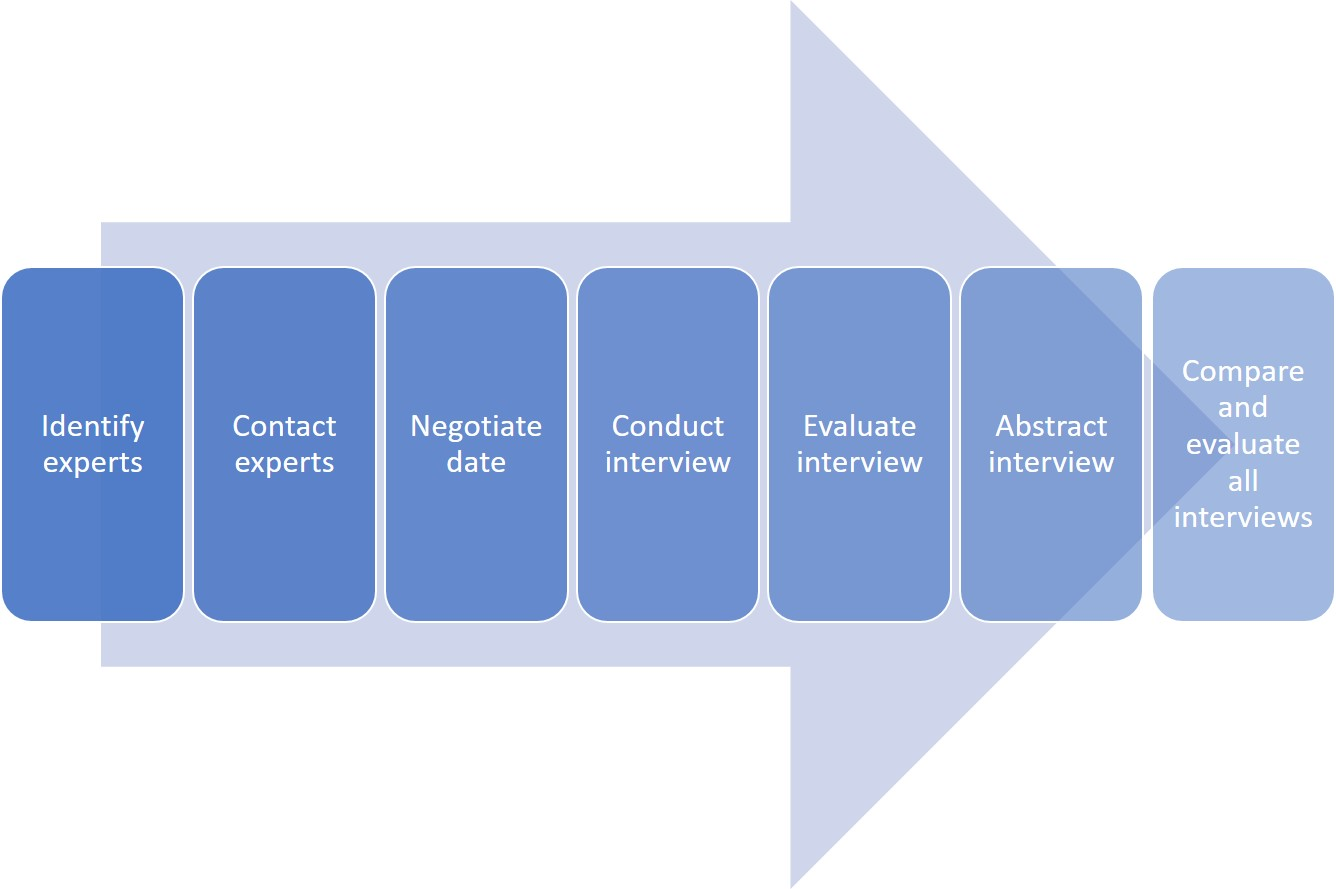
\includegraphics[width=1\textwidth]{Pictures/Interview_process}
	\caption{Interview process}
	\label{fig:Intprocess}
\end{figure}

\newpage

\paragraph{Identify experts} The experts are identified by conducting a network-based search. Initial contacts are asked to identify persons they consider an expert on the topic, who are in turn asked to provide further contacts.
\paragraph{Contact experts} Initial contact to the expert is established via an email sent by the expert's contact. Included is a standard email explaining the topic, duration and process of the interview and providing the researchers' contact details.
\paragraph{Negotiate date} Once the expert has agreed to participate in the interview, the researcher contacts them directly in order to set up date, time and method of communication for the interview. Note that all interviews are conducted using at least voice-based communication. Video can be added to further facilitate the communication between the expert and the researcher.
\paragraph{Conduct interview} The interviews are conducted in five phases with defined leading questions. This means, the leading questions will be asked, but the researcher will also ask further questions as appropriate to the course of the interview. These phases are:
\begin{itemize}
	\item Introduction
	\item Offshoring Experiences in the USA
	\item Offshoring Experiences in Germany
	\item Comparison of Experiences in Germany and the USA
	\item Finalization
\end{itemize}
During the interview, audio has been recorded. The audio files form the primary source of knowledge gained from the experts.


\paragraph{Evaluate interview} The recordings are evaluated and any important passages are noted. These evaluations are added to the appendix.

\paragraph{Abstract interview} For each interview, an abstract is developed. The abstracts are included in the thesis.

\paragraph{Compare and evaluate all interviews} Finally, an overview and comparison of all interviews is generated to derive common statements and areas of disagreement.

\newpage
\subsection{A German Project Manager on Offshoring with Different Service Providers}

This interview was conducted on 1. July 2016 08:00 h CEST with Michael Scheitza, a senior project manager at T-Systems International. The standard communication tool of T-Systems, Cisco WebEx, was used for the interview. The recording of the interview can be found on the enclosed CD (file name: 20160701\_Michael\_Scheitza.mp3). A written summary of the interview is found in appendix, page \pageref{int:Scheitza}.

\subsubsection{Background}
Michael Scheitza has worked for eight years as a project manager in an international environment. He has experience in offshoring projects with Russia, Poland, Romania, India, Malaysia, Mexico, and Brazil. He does not have any experience with offshoring from a U.S. perspective, so he did not feel comfortable answering any questions regarding this topic. 
\subsubsection{Results of Interview}
At T-Systems, application management contracts are often delivered offshore. Most customers leave the choice of delivery location to T-Systems, provided there is no legal obligation to deliver locally. The delivery model for each contract is chosen by the necessary skills, the language that is requested by the customer, and required service levels. When deciding on a delivery location, scalability is very important. It is essential that there are enough people with the required knowledge.

Generally speaking, there are two different possible working relationships between customer, German on-site team and offshore team. %Bilder hier einfügen

\vspace{3mm}
\begin{figure}[htbp]
	\centering
	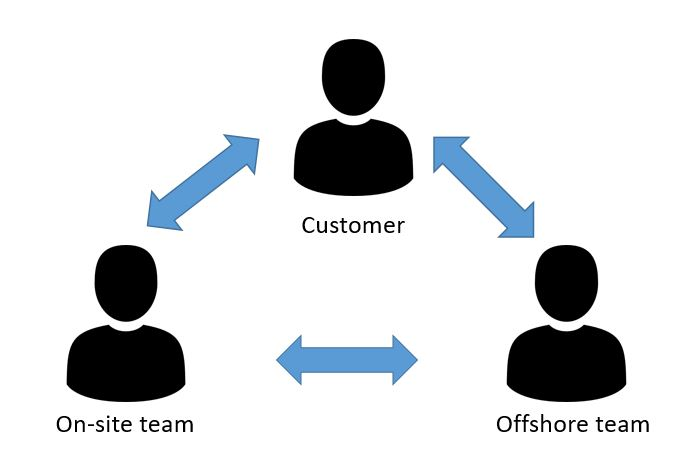
\includegraphics[width=0.5\textwidth]{Pictures/1on1_relationship}
	\caption{Direct, personal relationships between customer, on-site team and offshore team}
	\label{fig:1on1}
\end{figure}

The first possible working relationship works best in teams smaller than 50 persons offshore. In the transition phase, offshore team members travel to Germany in order to directly interact with and learn from the customer. In figure \ref{fig:1on1}, the set up in this case is depicted.

The interviewee gave an example of an application management contract that was delivered from Brazil. There was the requirement that all 20 team members speak enough German to directly speak to the customer. In transition phase, personal relationships were established between the Brazilian team, the customer and German project management of T-Systems. This facilitated collaboration later in the project, because the persons involved knew each other in person, not only via telephone and email.

The motivation for the offshore team in this case stems from the identification as part of a global delivery team. If the on-site and offshore teams share the same tasks, the delivery model is called \textit{Verl\"angerte Werkbank}. The team size in this case is usually less than 30 people and the project manager distributes tasks directly to offshore team members. 

The drawback in this approach is that it tends to increase volatility in the team. Michael Scheitza shared an experience he made with an Indian team: Each time there were quality issues, T-Systems had spent money on bringing team members on-site or German project management had traveled to India to improve communication. Few months later, he noticed that especially those team members who had been to Germany left the project and changed jobs in order to further their careers. This way, the investment in communication was unsuccessful.

\vspace{3mm}
\begin{figure}[htbp]
	\centering
	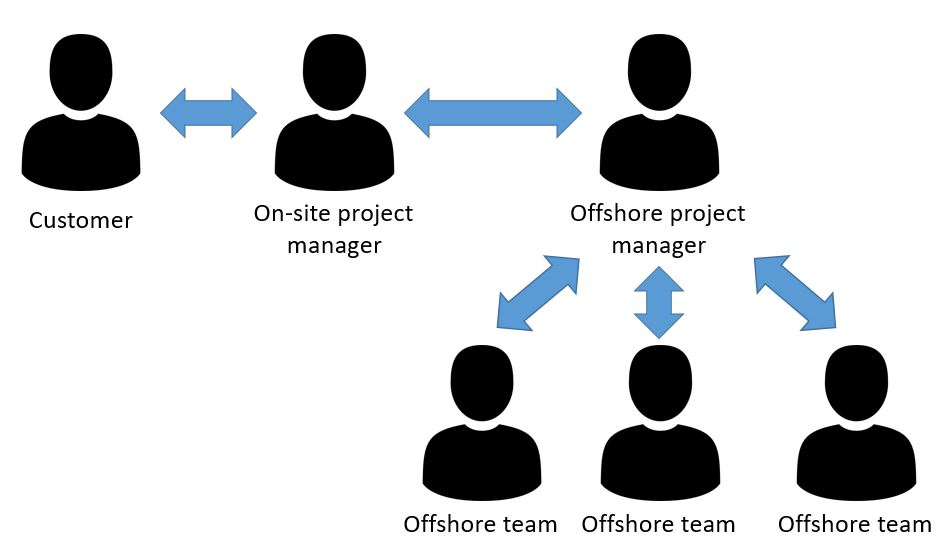
\includegraphics[width=0.7\textwidth]{Pictures/Hierarchy}
	\caption{Hierarchical communication between customer and offshore team}
	\label{fig:hierarchy}
\end{figure}

The second possibility is used in larger teams with more than 50 people. Teams that size are large enough to be organized in hierarchical layers with a local team lead or project management. This approach does not involve deep relationships and personal communication. Instead, the working relationship is managed via \glspl{sla} and \glspl{kpi}, where quality and quantity of deliverables are defined. The communication structure in this case is depicted in figure \ref{fig:hierarchy}. In transition phases of projects, only the offshore project managers or team leads travel to Germany and distribute the knowledge they gained in working with the customer to their teams offshore.

In this case, the offshore team does not identify as a part of a global delivery team, because the personal relationships that are needed for this approach are not in place. Alternately, the team members can identify with the project itself and are motivated by the local project manager. Ideally, the team is driven by the desire to be successful in fulfilling the contract.

Neither approach, said Michael Scheitza, is clearly superior to the other. Each has its drawbacks and advantages, and both are applicable in certain situations.

\subsubsection{Conclusions}

In the interview, Michael Scheitza differentiated and specified two distinct approaches to offshoring that are used in Germany. In table \ref{tab:ScheitzaApproaches}, they are directly compared to each other. 
\vspace{3mm}
\begin{table}[htb]
	\centering
	\begin{tabular}{l|p{5.8cm}|p{5.8cm}}
		& \textbf{Personal Relationships} & \textbf{Numbers-based Approach}\\\hline
		
		\rule{0pt}{3ex}Team size &$<$ 50 people &$>$ 50 people\\ \hline
		\rule{0pt}{3ex}Transition phase&All offshore team members travel on-site and form personal relationships with T-Systems team members and customers &Offshore project managers travel on-site and share their knowledge with the team\\ \hline
		\rule{0pt}{3ex}Communication &Direct communication between customer, on-site team and offshore team & Hierarchical communication from customer to on-site team to offshore project management to offshore team \\ \hline
		\rule{0pt}{3ex}Motivation &Identification as part of a global delivery team &Motivation by local project management and identification with the contract \\ \hline
	\end{tabular}
		\vspace{3mm}
		%Immer caption vor label!!!
		\caption{Comparison of German offshoring approaches according to M. Scheitza}
		\label{tab:ScheitzaApproaches}
\end{table}

Even though the interviewee could not contribute any experience with offshoring from an American point of view, there have been very interesting points. Firstly, the other interviews focused mainly on offshoring with an Indian service provider. This interview offered insights in offshoring projects with a multitude of different destinations. Secondly, there were criteria for choosing a delivery model outlined. Last, the two different collaboration models were described very thoroughly, offering a concise view on the offshoring projects the interviewee experienced.


\subsection{An Indian Offshoring Pioneer Comparing German and U.S. Clients}
A. S. Viswanathan agreed to an interview on 7. July 2016 at 17:00 h CEST / 20:30 h IST. For this, Skype was used as a communication tool. On the enclosed CD, the recording of the interview has the file name 20160707\_A\_S\_Viswanathan.mp3. The summary of the conversation can be found in appendix page \pageref{int:Viswanathan}.
\subsubsection{Background}
The interviewee is electrical engineer with a specialization in industrial engineering. In 1978, he started his career with English Electric, which was a part of General Electric Group. There, he worked for two years before joining Siemens. With Siemens, he held various positions ranging from the shop floor to CIO of the IT subsidiary of Siemens in India. Later, he moved on to the board of Siemens Information Systems, a software company that took global mandate within the Siemens Group. His responsibilities included Business Solutions for offshoring SAP, which his team was pioneering in India, as well as IT services.

In 2007, Siemens merged all local IT companies into a new company called IT Services and Solutions. Viswanathan was on the executive management of this company, heading Global Portfolio of Mobility.

After taking a break in 2011, he founded his own management consultation company in 2012. He specializes in offshoring consulting, primarily with customers from Germany, China and India.

\subsubsection{Results of Interview}
\paragraph{Offshoring in the US}When first conceptualizing the offer of offshoring services, the first customers were from the United States. They were very quick in understanding the advantages and seizing the opportunity, not only shifting single tasks, but entire operations to India. Before offshoring, U.S. companies took the time to evaluate different service providers. Once the decision was made, there was no plan B, so there was a necessity to make offshoring work.

This has a profound effect on working relationship. In Viswanathans experience, contributing to positive working relationships was English being a common language. Management meetings and schedules were easily set up. \Glspl{sla} were more critical, as after the initial cycles of new contracts, there would be a new wave of requirements, imposing stricter quality standards. In this phase, facts and figures dominate the working relationship.

The American approach to offshoring is characterized by legalistic and contractual concerns. When researching service providers, U.S. companies have consultants performing background searches of companies providing operations in India. Three to four companies are shortlisted and visited by the American team for presentations. Thereafter, contract negotiations start. A lot of emphasis is placed on contracting and commercial \glspl{sla}. The processes are not deemed as important, since the companies believed in the ability of the service provider to deliver.

Contributing to the success of American offshoring projects is the high offshorability of an American job. The work is conceptualized as a specific set of tasks where a specific set of skills is needed. Therefore, the skills of workforce can easily be managed. This goes back to U.S. companies already have experience with shifting jobs within the U.S. and people are already working in different places and time zones within the country. Also, jobs are very transaction-based in the U.S.. The education system facilitates that each employee does not need to have an end-to-end knowledge of the entire process. This is connected to the higher fluctuation of employees in American companies and is a huge advantage when it comes to offshoring -- it needs only minimal training to enable a new person to do the job.

\paragraph{Offshoring in Germany}Compared to American jobs, in German companies the job design is much more intrinsic and process-oriented. An example of a buyer is given: in Germany, the buyer has a specific background in the field, maybe an apprenticeship or some other kind of special training, whereas the buyer in the U.S. is not expected to have deep insights in the field when starting the job.

This kind of job design is mirrored in the SAP systems of companies. When it comes to customizing the system, a German system differs greatly from an American system, because the role of an individual is more holistic in Germany. This presents a problem when shifting tasks offshore, as one person in Germany can't simply be replaced by one equivalent person in India as it is the case with American jobs. The person in India simply lacks the specific background and experience with the German company.
	

\subsubsection{Conclusions}
\subsection{Ingo K\"ummritz}
\subsubsection{Background}
\subsubsection{Results of Interview}
\subsubsection{Conclusions}
\subsection{Subir Purkayastha}
\subsubsection{Background}
\subsubsection{Results of Interview}
\subsubsection{Conclusions}


\subsection{Summary and Evaluation}
